\documentclass[11pt,a4paper]{article}

% Packages
\usepackage[utf8]{inputenc}
\usepackage[T1]{fontenc}
\usepackage{lmodern}
\usepackage[margin=1in]{geometry}
\usepackage{hyperref}
\usepackage{listings}
\usepackage{xcolor}
\usepackage{graphicx}
\usepackage{tikz}
\usepackage{amsmath}
\usepackage{booktabs}
\usepackage{enumitem}
\usepackage{fancyhdr}
\usepackage{tocloft}

% Hyperref setup
\hypersetup{
    colorlinks=true,
    linkcolor=blue,
    filecolor=magenta,
    urlcolor=cyan,
}

% Code listing style
\definecolor{codebg}{RGB}{245,245,245}
\definecolor{codegreen}{RGB}{0,128,0}
\definecolor{codegray}{RGB}{128,128,128}
\definecolor{codepurple}{RGB}{128,0,128}

\lstdefinestyle{rustcode}{
    backgroundcolor=\color{codebg},
    basicstyle=\ttfamily\small,
    breakatwhitespace=false,
    breaklines=true,
    captionpos=b,
    commentstyle=\color{codegreen},
    keywordstyle=\color{blue}\bfseries,
    numberstyle=\tiny\color{codegray},
    stringstyle=\color{codepurple},
    showstringspaces=false,
    numbers=left,
    numbersep=5pt,
    frame=single,
    rulecolor=\color{black},
    tabsize=4,
}

\lstset{style=rustcode}

% Header/Footer
\pagestyle{fancy}
\fancyhf{}
\rhead{BetterSys Architecture}
\lhead{Rust Backend Overview}
\rfoot{Page \thepage}

% Title
\title{%
    \textbf{BetterSys: Rust Backend Architecture} \\
    \large A Comprehensive Technical Overview
}
\author{System Documentation}
\date{January 2026}

\begin{document}

\maketitle
\tableofcontents
\newpage

%==============================================================================
\section{Executive Summary}
%==============================================================================

BetterBot is a quantitative trading signal platform for Polymarket prediction markets. The Rust backend serves as the high-performance core, handling real-time data ingestion, signal detection, risk management, and automated trading execution.

\subsection{Technology Stack}

\begin{table}[h]
\centering
\begin{tabular}{@{}lll@{}}
\toprule
\textbf{Component} & \textbf{Technology} & \textbf{Purpose} \\
\midrule
Runtime & Tokio (async) & High-concurrency I/O \\
Web Framework & Axum 0.7 & HTTP/WebSocket API \\
Database & SQLite (WAL mode) & Signal persistence \\
Synchronization & parking\_lot & Fast locking primitives \\
Parallelism & Rayon & CPU-bound parallel processing \\
HTTP Client & reqwest (rustls) & External API calls \\
WebSocket & tokio-tungstenite & Real-time streaming \\
\bottomrule
\end{tabular}
\caption{Core Technology Stack}
\end{table}

%==============================================================================
\section{Directory Structure}
%==============================================================================

The backend follows a modular architecture with clear separation of concerns:

\begin{lstlisting}[language=bash,caption={Source Directory Layout}]
rust-backend/src/
|-- main.rs           # Entry point, server orchestration
|-- models.rs         # Core data structures
|-- risk.rs           # Kelly criterion, VaR calculations
|-- backtest.rs       # Historical signal analysis
|-- api/              # HTTP REST endpoints
|   |-- mod.rs
|   |-- simple.rs     # Main API handlers
|   |-- routes.rs
|-- auth/             # JWT authentication
|   |-- mod.rs
|   |-- jwt.rs
|   |-- middleware.rs
|   |-- user_store.rs
|-- scrapers/         # External API integrations
|   |-- mod.rs
|   |-- dome_websocket.rs
|   |-- dome_rest.rs
|   |-- polymarket_api.rs
|   |-- binance_price_feed.rs
|   |-- hashdive_api.rs
|-- signals/          # Signal detection & storage
|   |-- mod.rs
|   |-- detector.rs
|   |-- db_storage.rs
|   |-- enrichment.rs
|   |-- wallet_analytics.rs
|-- vault/            # Auto-trading infrastructure
|   |-- mod.rs
|   |-- engine.rs
|   |-- kelly.rs
|   |-- pool.rs
|   |-- paper_ledger.rs
|   |-- llm.rs
|-- arbitrage/        # Cross-platform arbitrage
    |-- mod.rs
    |-- engine.rs
\end{lstlisting}

%==============================================================================
\section{Core Modules}
%==============================================================================

\subsection{Main Entry Point (main.rs)}

The entry point orchestrates the entire application lifecycle:

\subsubsection{AppState Structure}
\begin{lstlisting}[language=Rust,caption={Shared Application State}]
struct AppState {
    signal_storage: Arc<DbSignalStorage>,
    risk_manager: Arc<ParkingRwLock<RiskManager>>,
    signal_broadcast: broadcast::Sender<WsServerEvent>,
    http_client: reqwest::Client,
    dome_rest: Option<Arc<DomeRestClient>>,
    polymarket_market_ws: Arc<PolymarketMarketWsCache>,
    binance_feed: Arc<BinancePriceFeed>,
    vault: Arc<PooledVault>,
}
\end{lstlisting}

\subsubsection{Background Tasks}
The main function spawns several concurrent polling tasks:
\begin{itemize}
    \item \texttt{parallel\_data\_collection()} -- 45-minute Polymarket/Hashdive/Dome polling
    \item \texttt{tracked\_wallet\_polling()} -- Dome WebSocket + REST for tracked wallets
    \item \texttt{expiry\_edge\_polling()} -- 60-second market expiry scanner
    \item \texttt{wallet\_analytics\_polling()} -- Cache warming for wallet analytics
    \item \texttt{storage\_pruning\_polling()} -- Database maintenance
    \item \texttt{search\_index\_backfill\_polling()} -- FTS5 index population
\end{itemize}

\subsubsection{Kill-Switch Pattern}
Each data source has a health monitor with automatic disable:
\begin{lstlisting}[language=Rust,caption={Data Source Kill-Switch}]
struct DataSourceKillSwitch {
    name: &'static str,
    enabled: bool,
    kill_triggered: bool,
    failure_threshold: u32,
    latency_threshold_ms: f64,
    consecutive_failures: u32,
    latencies_ms: VecDeque<f64>,
}
\end{lstlisting}

%==============================================================================
\subsection{Data Models (models.rs)}

\subsubsection{MarketSignal}
The core signal structure used throughout the system:
\begin{lstlisting}[language=Rust,caption={Market Signal Structure}]
pub struct MarketSignal {
    pub id: String,
    pub signal_type: SignalType,
    pub market_slug: String,
    pub confidence: f64,
    pub risk_level: String,
    pub details: SignalDetails,
    pub detected_at: String,
    pub source: String,
}
\end{lstlisting}

\subsubsection{SignalType Variants}
Signals are categorized using a tagged union:
\begin{itemize}
    \item \texttt{PriceDeviation} -- Market price vs fair value divergence
    \item \texttt{MarketExpiryEdge} -- Near-expiry high-probability markets
    \item \texttt{WhaleFollowing} -- Large position tracking
    \item \texttt{EliteWallet} -- High win-rate trader activity
    \item \texttt{InsiderWallet} -- Early-entry pattern detection
    \item \texttt{TrackedWalletEntry} -- Real-time wallet order signals
    \item \texttt{CrossPlatformArbitrage} -- Multi-platform price discrepancies
\end{itemize}

\subsubsection{Tracked Wallet Taxonomy}
The system tracks approximately 384 wallets across categories:
\begin{table}[h]
\centering
\begin{tabular}{@{}lr@{}}
\toprule
\textbf{Category} & \textbf{Count} \\
\midrule
insider\_politics & 134 \\
insider\_finance & 65 \\
insider\_entertainment & 39 \\
insider\_crypto & 23 \\
insider\_sports & 5 \\
insider\_tech & varies \\
high\_frequency\_test & 1 \\
\bottomrule
\end{tabular}
\caption{Tracked Wallet Distribution}
\end{table}

%==============================================================================
\subsection{Risk Management (risk.rs)}

\subsubsection{Kelly Criterion Implementation}
The system uses fractional Kelly for position sizing:

\begin{equation}
f^* = \frac{p \cdot b - q}{b}
\end{equation}

where:
\begin{itemize}
    \item $f^*$ = optimal fraction of bankroll
    \item $p$ = probability of winning
    \item $q = 1 - p$ = probability of losing
    \item $b$ = odds ratio $(1/p) - 1$
\end{itemize}

\begin{lstlisting}[language=Rust,caption={Kelly Calculator}]
pub struct KellyCalculator {
    pub fraction: f64,      // Safety multiplier (0.25-0.5x)
    pub bankroll: f64,
    win_history: VecDeque<bool>,
}

impl KellyCalculator {
    pub fn raw_fraction(&self, win_probability: f64) -> f64 {
        let p = win_probability.clamp(0.001, 0.999);
        let q = 1.0 - p;
        let b = (1.0 / p) - 1.0;
        ((b * p - q) / b).max(0.0)
    }
}
\end{lstlisting}

\subsubsection{Value at Risk (VaR)}
Historical simulation VaR at 95\% and 99\% confidence:
\begin{lstlisting}[language=Rust,caption={VaR Calculator}]
pub struct VaRCalculator {
    historical_pnl: VecDeque<f64>,
    confidence_level: f64,  // 0.95 or 0.99
}
\end{lstlisting}

\subsubsection{Guardrails}
Multiple safety mechanisms prevent excessive risk:
\begin{itemize}
    \item Maximum Kelly cap: 20\%
    \item Drawdown throttle trigger: 8\%
    \item Drawdown throttle release: 4\%
    \item Liquidity factor scaling
    \item Per-signal-family calibration
\end{itemize}

%==============================================================================
\section{API Module}
%==============================================================================

\subsection{Route Summary}

\begin{table}[h]
\centering
\small
\begin{tabular}{@{}llp{6cm}@{}}
\toprule
\textbf{Method} & \textbf{Endpoint} & \textbf{Description} \\
\midrule
GET & /health & Health check \\
POST & /api/auth/login & JWT login \\
GET & /api/signals & Signal list (protected) \\
GET & /api/signals/search & FTS5 full-history search \\
GET & /api/signals/enrich & 15m Up/Down enrichment \\
GET & /api/market/snapshot & Orderbook snapshot \\
GET & /api/wallet/analytics & Wallet performance curves \\
GET & /api/vault/state & Pooled vault state \\
POST & /api/vault/deposit & Mint vault shares \\
POST & /api/vault/withdraw & Burn vault shares \\
POST & /api/trade/order & One-click trade (feature-flagged) \\
GET & /ws & WebSocket upgrade \\
\bottomrule
\end{tabular}
\caption{API Endpoints}
\end{table}

\subsection{Signal Response Structure}
\begin{lstlisting}[language=Rust,caption={Signal API Response}]
pub struct SignalResponse {
    pub signals: Vec<SignalWithContext>,
    pub count: usize,
    pub timestamp: String,
}

pub struct SignalWithContext {
    pub signal: MarketSignal,
    pub context: Option<SignalContext>,
    pub context_status: Option<String>,
    pub context_version: Option<i64>,
}
\end{lstlisting}

%==============================================================================
\section{Scrapers Module}
%==============================================================================

\subsection{Data Sources}

\begin{table}[h]
\centering
\begin{tabular}{@{}llll@{}}
\toprule
\textbf{Source} & \textbf{Protocol} & \textbf{Frequency} & \textbf{Purpose} \\
\midrule
Polymarket GAMMA & REST & 45 min & Market data, events \\
Polymarket CLOB & REST/WS & On-demand & Orderbook snapshots \\
Hashdive & REST & 45 min & Whale trades (\$10k+) \\
DomeAPI WS & WebSocket & Real-time & Wallet order streaming \\
DomeAPI REST & REST & 30s fallback & Order history \\
Binance & WebSocket & Real-time & BTC/ETH/SOL/XRP prices \\
\bottomrule
\end{tabular}
\caption{External Data Sources}
\end{table}

\subsection{Dome WebSocket Client}

The primary real-time feed for tracked wallet orders:

\begin{lstlisting}[language=Rust,caption={Dome WebSocket Subscription}]
pub struct WsSubscribeMessage {
    pub action: String,        // "subscribe"
    pub platform: String,      // "polymarket"
    pub version: i32,          // 1
    pub msg_type: String,      // "orders"
    pub filters: WsFilters,    // { users: ["0x..."] }
}
\end{lstlisting}

Features:
\begin{itemize}
    \item Auto-reconnect with exponential backoff (1s to 60s)
    \item TLS via rustls-tls-webpki-roots
    \item Subscription to 384+ wallets
    \item Sub-second latency for order detection
\end{itemize}

\subsection{Binance Price Feed}

Real-time L1 orderbook streaming via \texttt{barter-data}:

\begin{lstlisting}[language=Rust,caption={Binance Price Feed}]
pub struct BinancePriceFeed {
    inner: Arc<RwLock<HashMap<String, SymbolState>>>,
    max_history_len: usize,  // ~3h at 1Hz
    ewma_lambda: f64,        // 0.97
}
\end{lstlisting}

Capabilities:
\begin{itemize}
    \item BTCUSDT, ETHUSDT, SOLUSDT, XRPUSDT L1 books
    \item Historical mid-price lookup with time tolerance
    \item EWMA volatility estimation ($\sigma$ per $\sqrt{\text{second}}$)
\end{itemize}

%==============================================================================
\section{Signals Module}
%==============================================================================

\subsection{Database Storage (db\_storage.rs)}

SQLite with aggressive optimizations for 10M+ signal capacity:

\begin{lstlisting}[language=SQL,caption={SQLite Performance Pragmas}]
PRAGMA journal_mode = WAL;
PRAGMA synchronous = NORMAL;
PRAGMA cache_size = -64000;     -- 64MB
PRAGMA mmap_size = 268435456;   -- 256MB
\end{lstlisting}

\subsubsection{Schema Tables}
\begin{itemize}
    \item \texttt{signals} -- Core signal storage (WITHOUT ROWID, clustered)
    \item \texttt{signal\_context} -- Enrichment payloads
    \item \texttt{signal\_search} -- FTS5 content table
    \item \texttt{signal\_search\_fts} -- FTS5 virtual table
    \item \texttt{dome\_order\_events} -- Raw order payloads
    \item \texttt{dome\_cache} -- DB-backed API cache
    \item \texttt{vault\_llm\_decisions} -- LLM decision audit log
\end{itemize}

\subsubsection{Full-Text Search}
FTS5-backed search with incremental backfill:
\begin{lstlisting}[language=SQL,caption={FTS5 Virtual Table}]
CREATE VIRTUAL TABLE signal_search_fts USING fts5(
    market_slug,
    market_title,
    wallet_address,
    wallet_label,
    token_label,
    source,
    signal_type,
    content='signal_search',
    tokenize='unicode61 remove_diacritics 2'
);
\end{lstlisting}

\subsection{Signal Detector}

Detection pipeline for multiple signal types:

\begin{lstlisting}[language=Rust,caption={Signal Detector}]
pub struct SignalDetector {
    confidence_threshold: f64,  // 0.6
}

impl SignalDetector {
    pub async fn detect_all(&self, events: &[PolymarketEvent]) 
        -> Vec<MarketSignal>;
    
    pub fn detect_trader_entry(
        &self,
        orders: &[DomeOrder],
        wallet_address: &str,
        wallet_label: &str,
    ) -> Vec<MarketSignal>;
}
\end{lstlisting}

\subsubsection{Confidence Scoring}
Tracked wallet confidence by category:
\begin{table}[h]
\centering
\begin{tabular}{@{}lr@{}}
\toprule
\textbf{Wallet Label} & \textbf{Base Confidence} \\
\midrule
insider\_politics & 0.90 \\
insider\_finance & 0.88 \\
insider\_tech & 0.87 \\
insider\_crypto & 0.86 \\
insider\_sports & 0.85 \\
insider\_entertainment & 0.84 \\
high\_frequency\_test & 0.50 \\
\bottomrule
\end{tabular}
\caption{Confidence by Wallet Category}
\end{table}

%==============================================================================
\section{Vault Module}
%==============================================================================

\subsection{Architecture Overview}

The vault implements pooled share-based accounting with automated trading:

\begin{lstlisting}[language=Rust,caption={Pooled Vault Structure}]
pub struct PooledVault {
    pub db: Arc<VaultDb>,
    pub ledger: Arc<Mutex<VaultPaperLedger>>,
    pub shares: Arc<Mutex<VaultShareState>>,
}

pub struct VaultShareState {
    pub total_shares: f64,
    pub user_shares: HashMap<String, f64>,
}
\end{lstlisting}

\subsection{Trading Engines}

\subsubsection{FAST15M Engine}
Deterministic 15-minute Up/Down markets:
\begin{itemize}
    \item Assets: BTC, ETH, SOL, XRP
    \item Price source: Binance mid via \texttt{barter-data}
    \item Probability model: Driftless lognormal
    \item Position sizing: Fractional Kelly with shrink-to-half
\end{itemize}

\begin{equation}
P(\text{Up}) = \Phi\left(\frac{\ln(S_t / S_0)}{\sigma \sqrt{T - t}}\right)
\end{equation}

\subsubsection{LONG Engine (LLM-Bounded)}
Non-deterministic markets with LLM consensus:
\begin{itemize}
    \item Scout-first gating (first model must pass)
    \item 3-of-4 model consensus required
    \item Daily budget limits: calls, tokens
    \item Per-market cadence enforcement
\end{itemize}

\begin{lstlisting}[language=Rust,caption={LONG Engine Configuration}]
pub struct VaultEngineConfig {
    pub long_enabled: bool,
    pub long_max_calls_per_day: u32,        // 200
    pub long_max_tokens_per_day: u64,       // 300,000
    pub long_max_calls_per_market_per_day: u32,  // 30
    pub long_models: Vec<String>,           // 4 models
}
\end{lstlisting}

\subsection{Execution Adapters}

\begin{lstlisting}[language=Rust,caption={Execution Adapter Trait}]
pub trait ExecutionAdapter: Send + Sync {
    async fn place_order(&self, req: OrderRequest) 
        -> Result<OrderResponse>;
    async fn cancel_order(&self, order_id: &str) 
        -> Result<()>;
}
\end{lstlisting}

Implementations:
\begin{itemize}
    \item \texttt{PaperExecutionAdapter} -- Instant fills at limit price
    \item \texttt{DomeExecutionAdapter} -- Placeholder for live execution
\end{itemize}

%==============================================================================
\section{Authentication Module}
%==============================================================================

\subsection{JWT Authentication}

\begin{lstlisting}[language=Rust,caption={JWT Handler}]
pub struct JwtHandler {
    secret: String,
    // Token validation and generation
}

pub async fn auth_middleware(
    State(jwt): State<Arc<JwtHandler>>,
    request: Request,
    next: Next,
) -> Response;
\end{lstlisting}

\subsection{User Store}
SQLite-backed user management with bcrypt password hashing:
\begin{lstlisting}[language=SQL,caption={Auth Schema}]
CREATE TABLE users (
    id INTEGER PRIMARY KEY,
    username TEXT UNIQUE NOT NULL,
    password_hash TEXT NOT NULL,  -- bcrypt, cost 12
    created_at TEXT NOT NULL
);
\end{lstlisting}

%==============================================================================
\section{Data Flow Architecture}
%==============================================================================

\begin{figure}[h]
\centering
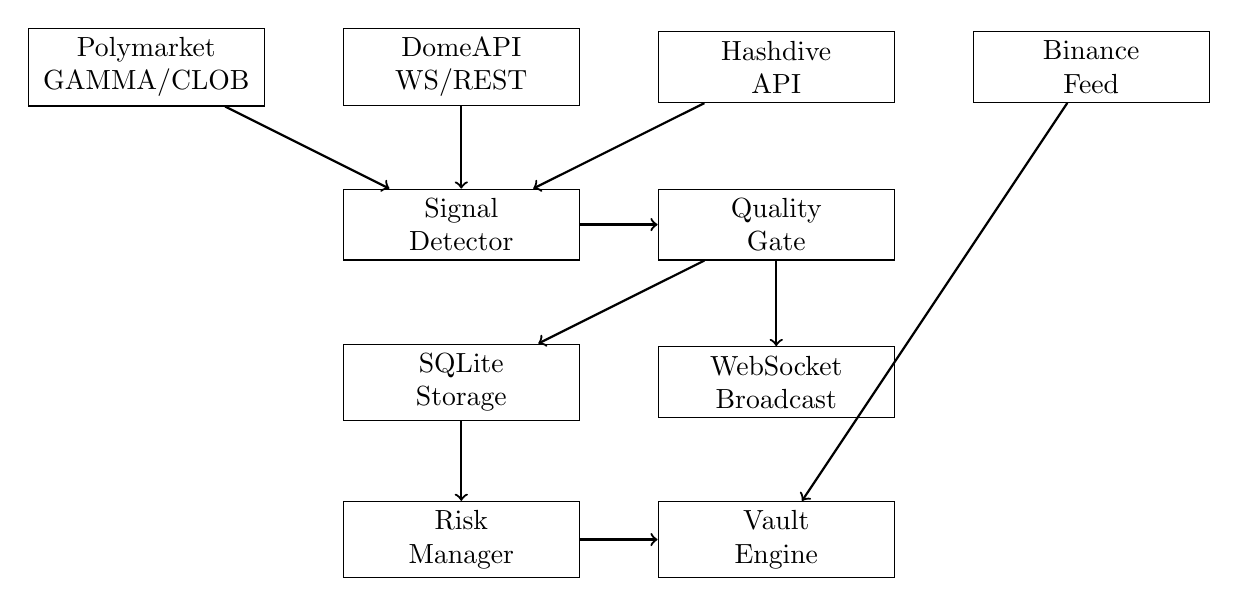
\begin{tikzpicture}[
    box/.style={rectangle, draw, minimum width=3cm, minimum height=0.8cm, align=center},
    arrow/.style={->, thick},
]
    % Data Sources
    \node[box] (poly) at (0,4) {Polymarket\\GAMMA/CLOB};
    \node[box] (dome) at (4,4) {DomeAPI\\WS/REST};
    \node[box] (hash) at (8,4) {Hashdive\\API};
    \node[box] (binance) at (12,4) {Binance\\Feed};
    
    % Detection
    \node[box] (detector) at (4,2) {Signal\\Detector};
    \node[box] (quality) at (8,2) {Quality\\Gate};
    
    % Storage & Broadcast
    \node[box] (storage) at (4,0) {SQLite\\Storage};
    \node[box] (broadcast) at (8,0) {WebSocket\\Broadcast};
    
    % Risk & Vault
    \node[box] (risk) at (4,-2) {Risk\\Manager};
    \node[box] (vault) at (8,-2) {Vault\\Engine};
    
    % Arrows
    \draw[arrow] (poly) -- (detector);
    \draw[arrow] (dome) -- (detector);
    \draw[arrow] (hash) -- (detector);
    \draw[arrow] (binance) -- (vault);
    \draw[arrow] (detector) -- (quality);
    \draw[arrow] (quality) -- (storage);
    \draw[arrow] (quality) -- (broadcast);
    \draw[arrow] (storage) -- (risk);
    \draw[arrow] (risk) -- (vault);
\end{tikzpicture}
\caption{Signal Processing Pipeline}
\end{figure}

%==============================================================================
\section{Environment Configuration}
%==============================================================================

\subsection{Required Variables}

\begin{lstlisting}[language=bash,caption={Essential Environment Variables}]
# Database
DATABASE_PATH=betterbot_signals.db
AUTH_DB_PATH=betterbot_auth.db
VAULT_DB_PATH=betterbot_vault.db

# API Keys
DOME_API_KEY=<bearer_token>
HASHDIVE_API_KEY=<api_key>

# Risk
INITIAL_BANKROLL=10000
KELLY_FRACTION=0.25

# JWT
JWT_SECRET=<min-32-chars>

# Features
VAULT_ENGINE_ENABLED=false
VAULT_ENGINE_PAPER=true
ENABLE_TRADING=false
\end{lstlisting}

\subsection{Optional Tuning}

\begin{lstlisting}[language=bash,caption={Optional Configuration}]
# Polling intervals
POLL_INTERVAL_SECS=2700
WALLET_ANALYTICS_POLL_SECS=3600

# FAST15M tuning
UPDOWN15M_POLL_MS=2000
UPDOWN15M_MIN_EDGE=0.01
UPDOWN15M_KELLY_FRACTION=0.05

# LONG (LLM) tuning
VAULT_LLM_ENABLED=false
VAULT_LLM_MAX_CALLS_PER_DAY=200
VAULT_LLM_MAX_TOKENS_PER_DAY=300000
OPENROUTER_API_KEY=<key>
\end{lstlisting}

%==============================================================================
\section{Performance Optimizations}
%==============================================================================

\begin{table}[h]
\centering
\begin{tabular}{@{}llp{6cm}@{}}
\toprule
\textbf{Optimization} & \textbf{Location} & \textbf{Impact} \\
\midrule
parking\_lot::RwLock & main.rs & 2-5x faster than std \\
WAL mode + 64MB cache & db\_storage.rs & 10x write throughput \\
Batch inserts & db\_storage.rs & 100x faster bulk storage \\
Connection pooling & scrapers & Reduced TCP overhead \\
Pre-allocated vectors & All modules & Fewer allocations \\
WITHOUT ROWID tables & Schema & Clustered primary keys \\
Covering indexes & Schema & Index-only scans \\
\bottomrule
\end{tabular}
\caption{Backend Optimizations}
\end{table}

\subsection{Measured Performance}
\begin{itemize}
    \item API latency: 8-9ms average (sub-10ms target achieved)
    \item Database capacity: 10M+ signals
    \item Memory: Stable under continuous operation
    \item WebSocket: Sub-second signal delivery
\end{itemize}

%==============================================================================
\section{Conclusion}
%==============================================================================

The BetterSys Rust backend provides a high-performance foundation for quantitative trading on Polymarket. Key architectural decisions include:

\begin{enumerate}
    \item \textbf{Async-first design} with Tokio for maximum concurrency
    \item \textbf{SQLite with WAL mode} for simplicity and performance
    \item \textbf{Kill-switch pattern} for resilient data source management
    \item \textbf{Fractional Kelly} with multiple guardrails for risk control
    \item \textbf{Paper-first execution} for safe development and testing
    \item \textbf{LLM consensus} for non-deterministic market evaluation
\end{enumerate}

The modular design allows independent evolution of scraping, detection, risk management, and execution components while maintaining a unified signal pipeline.

\end{document}
